\section{ \bfseries Markowitz Portfolio Optimization}
This exercise illustrates use of quadratic programming in a financial application. By diversifying an investment into several securities it may be possible to reduce risk without reducing return. Identification and construction of such portfolios is called hedging. The Markowitz Portofolio Optimization problem is very simple hedging problem for
which Markowitz was awarded the Nobel Price in 1990.\\[0.3cm]
Consider a financial market with 5 securities.\\[0.3cm]
\begin{tabular}{c|ccccc|c}
\hline Security & \multicolumn{5}{|c|} { Covariance } &  Return\\
\hline 1 & 2.30 & 0.93 & 0.62 & 0.74 & -0.23 & 15.10 \\
2 & 0.93 & 1.40 & 0.22 & 0.56 & 0.26 & 12.50 \\
3 & 0.62 & 0.22 & 1.80 & 0.78 & -0.27 & 14.70 \\
4 & 0.74 & 0.56 & 0.78 & 3.40 & -0.56 & 9.02 \\
5 & -0.23 & 0.26 & -0.27 & -0.56 & 2.60 & 17.68 \\
\hline
\end{tabular}

%%%%%%%%%%%%%%%%%%%%%%%%%%%%%%%%%%%%%%%%%%
%%%%%%%%%%%%%%%%%%%%%%%%%%%%%%%%%%%%%%%%%%%%%%%%%%%%%%%%%%%%%%%%%%%%%%%%%%%%%%%%%%%%%
%%%%%%%%%%%%%%%%%%%%%%%%%%%%%%%%%%%%%%%%%%%
%%%%%%%%%%%%%%%%%%%%%%%%%%%%%%%%%%%%%%%%%%
%%%%%%%%%%%%%%%%%%%%%%%%%%%%%%%%%%%%%%%%%%%
\subsection{\bfseries Original problem}
%%%%%%%%%%%%%%%%%%%%%%%%%%%%%%%%%%%%%%%%%%
%%%%%%%%%%%%%%%%%%%%%%%%%%%%%%%%%%%%%%%%%%%%%%%%%%%%%%%%%%%%%%%%%%%%%%%%%%%%%%%%%%%%%
%%%%%%%%%%%%%%%%%%%%%%%%%%%%%%%%%%%%%%%%%%%
%%%%%%%%%%%%%%%%%%%%%%%%%%%%%%%%%%%%%%%%%%
%%%%%%%%%%%%%%%%%%%%%%%%%%%%%%%%%%%%%%%%%%%
\subsubsection{\bfseries Formulation}
\begin{shaded}
{ Question: For a given return, $R$, formulate Markowitz’ Portfolio optimization problem as a quadratic program.}
\end{shaded}
\begin{align*}
&\min_{x \in \mathcal{R}^n} \quad \phi=\frac{1}{2}x^{\prime}Hx \tag{3}\\
& s.t. \quad \mu^{\prime}x\ge R\\
& \quad \quad \sum_{i=1}^{n}x_i=1\\
& \quad \quad \ x \ge 0
\end{align*}
Required return is $R$, expected return and variance of the portfolio\\
\begin{align*}
\bar{R}=E\{ R\}&=E\{ r^{\prime}x\}=\mu^{\prime}x \tag{3.1}\\
 V\{ R\}&=E\{(R-\bar{R})^2 \}=E{x^{\prime}(r-\mu)(r-\mu)^{\prime}x}=x^{\prime}Hx \tag{3.2}\\
\end{align*}

%%%%%%%%%%%%%%%%%%%%%%%%%%%%%%%%%%%%%%%%%%
%%%%%%%%%%%%%%%%%%%%%%%%%%%%%%%%%%%%%%%%%%%%%%%%%%%%%%%%%%%%%%%%%%%%%%%%%%%%%%%%%%%%%
%%%%%%%%%%%%%%%%%%%%%%%%%%%%%%%%%%%%%%%%%%%
%%%%%%%%%%%%%%%%%%%%%%%%%%%%%%%%%%%%%%%%%%
%%%%%%%%%%%%%%%%%%%%%%%%%%%%%%%%%%%%%%%%%%%
\subsubsection{\bfseries Minimal and maximal return}
\begin{shaded}
{ Question: What is the minimal and maximal possible return in this financial market?}
\end{shaded}
If the variance of the protfolio is not considered, the security 4 can only be invested to obtain the minimal return 9.02, or only invest in security 5 to obtain maximal return 17.68.
%%%%%%%%%%%%%%%%%%%%%%%%%%%%%%%%%%%%%%%%%%
%%%%%%%%%%%%%%%%%%%%%%%%%%%%%%%%%%%%%%%%%%%%%%%%%%%%%%%%%%%%%%%%%%%%%%%%%%%%%%%%%%%%%
%%%%%%%%%%%%%%%%%%%%%%%%%%%%%%%%%%%%%%%%%%%
%%%%%%%%%%%%%%%%%%%%%%%%%%%%%%%%%%%%%%%%%%
%%%%%%%%%%%%%%%%%%%%%%%%%%%%%%%%%%%%%%%%%%%
\subsubsection{\bfseries Optimal
portfolio}
\begin{shaded}
{ Question: Compute a portfolio with return, $R = 10.0$, and minimal risk. What is the optimal portfolio and what is the risk (variance)?}
\end{shaded}
To achieve a return of exactly 10 then the constraint $\mu^{\prime}x\ge R$ have to be changed to an equlity constraint $\mu^{\prime}x= R$. The Matlab function $quadprog$ is used to solve the constructed problem. Please see the driver files in appendix \ref{6.3.1}. The calculated optimal portfolio is 
\begin{align*}
&    x=(0,0.2816,0,0.7184,0)^{\prime}\\
&Return: \quad E\{ R\}=10\\
&Risk(Variance):\quad V\{ R\}=x^{\prime}Hx=2.0923
\end{align*}

However, the highest possible return with the minimum variance is generally desired. The original constraint is maintained  $\mu^{\prime}x\ge R$ to get the highest possible return and greater than 10. Please see the driver files in appendix \ref{6.3.2}. The optimal portfolio is 
 \begin{align*}
&    x=(0.0883,0.2509,0.2824,0.1038,0.2748)^{\prime}\\
&Return: \quad E\{ R\}=14.4129\\
&Risk(Variance):\quad V\{ R\}=x^{\prime}Hx=0.6249
\end{align*}
%%%%%%%%%%%%%%%%%%%%%%%%%%%%%%%%%%%%%%%%%%
%%%%%%%%%%%%%%%%%%%%%%%%%%%%%%%%%%%%%%%%%%%%%%%%%%%%%%%%%%%%%%%%%%%%%%%%%%%%%%%%%%%%%
%%%%%%%%%%%%%%%%%%%%%%%%%%%%%%%%%%%%%%%%%%%
%%%%%%%%%%%%%%%%%%%%%%%%%%%%%%%%%%%%%%%%%%
%%%%%%%%%%%%%%%%%%%%%%%%%%%%%%%%%%%%%%%%%%%
\subsubsection{\bfseries Efficient frontier}
\begin{shaded}
{ Question:  Compute the efficient frontier, i.e. the risk as function of the return. Plot the efficient frontier as well as the optimal portfolio as function of return.}
\end{shaded}
\begin{figure}[H]
\centering
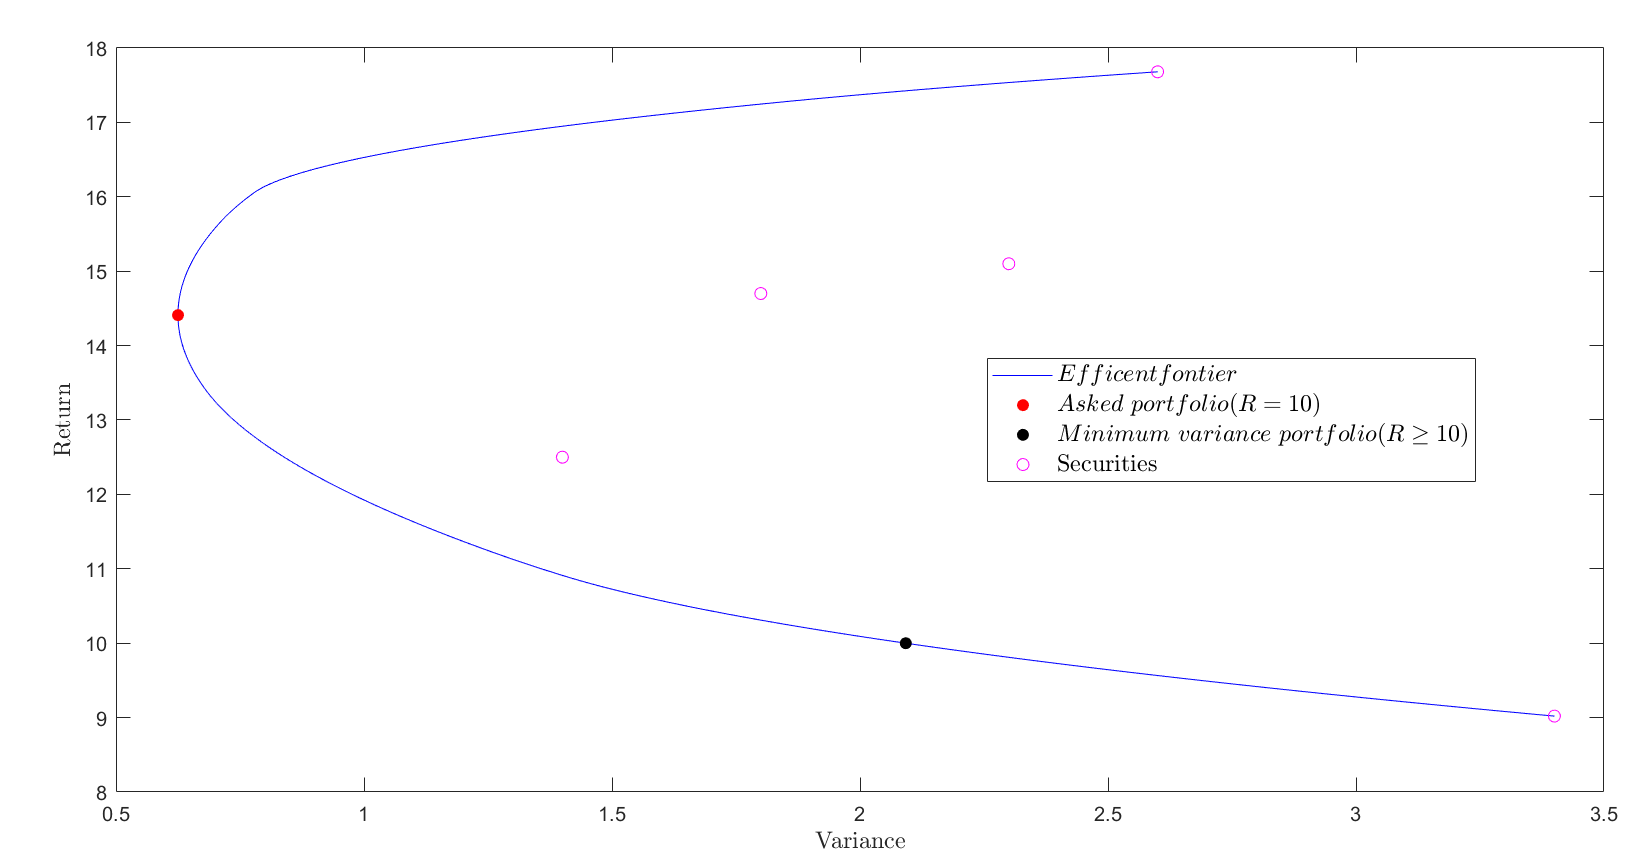
\includegraphics[scale=0.5]{figures/eff_fro1.PNG}
\caption{Efficient frontier of the portfolio}
\label{fig:labe3.1.4}
\end{figure}
Where the black filled dot is the asked portfolio($R=10$), and the red filled dot is the minimum variance and the return is also satisfied the asked portfolio. The pink unfilled dot is the securities. Please see the driver files in appendix \ref{6.3.3}.

%%%%%%%%%%%%%%%%%%%%%%%%%%%%%%%%%%%%%%%%%%
%%%%%%%%%%%%%%%%%%%%%%%%%%%%%%%%%%%%%%%%%%%%%%%%%%%%%%%%%%%%%%%%%%%%%%%%%%%%%%%%%%%%%
%%%%%%%%%%%%%%%%%%%%%%%%%%%%%%%%%%%%%%%%%%%
%%%%%%%%%%%%%%%%%%%%%%%%%%%%%%%%%%%%%%%%%%
%%%%%%%%%%%%%%%%%%%%%%%%%%%%%%%%%%%%%%%%%%%
\newpage
\subsection{\bfseries Problem with an added risk free security}
%%%%%%%%%%%%%%%%%%%%%%%%%%%%%%%%%%%%%%%%%%
%%%%%%%%%%%%%%%%%%%%%%%%%%%%%%%%%%%%%%%%%%%%%%%%%%%%%%%%%%%%%%%%%%%%%%%%%%%%%%%%%%%%%
%%%%%%%%%%%%%%%%%%%%%%%%%%%%%%%%%%%%%%%%%%%
%%%%%%%%%%%%%%%%%%%%%%%%%%%%%%%%%%%%%%%%%%
%%%%%%%%%%%%%%%%%%%%%%%%%%%%%%%%%%%%%%%%%%%
\subsubsection{\bfseries New covariance matrix and return vector}
\begin{shaded}
{ Question: What is the new covariance matrix and return vector}
\end{shaded}
The new covariance matrix and return vector is
$$H=\begin{bmatrix}
2.30 & 0.93 & 0.62 & 0.74 & -0.23 & 0 \\
0.93 & 1.40 & 0.22 & 0.56 & 0.26 & 0 \\
0.62 & 0.22 & 1.80 & 0.78 & -0.27 & 0 \\
0.74 & 0.56 & 0.78 & 3.40 & -0.56 & 0 \\
-0.23 & 0.26 & -0.27 & -0.56 & 2.60 & 0 \\
0 & 0 & 0 & 0 & 0 &0
\end{bmatrix}\quad \mu=\begin{bmatrix}
15.10\\
12.50\\
14.70\\
9.02\\
17.68\\
2.0
\end{bmatrix}$$
%%%%%%%%%%%%%%%%%%%%%%%%%%%%%%%%%%%%%%%%%%
%%%%%%%%%%%%%%%%%%%%%%%%%%%%%%%%%%%%%%%%%%%%%%%%%%%%%%%%%%%%%%%%%%%%%%%%%%%%%%%%%%%%%
%%%%%%%%%%%%%%%%%%%%%%%%%%%%%%%%%%%%%%%%%%%
%%%%%%%%%%%%%%%%%%%%%%%%%%%%%%%%%%%%%%%%%%
%%%%%%%%%%%%%%%%%%%%%%%%%%%%%%%%%%%%%%%%%%%
\subsubsection{\bfseries Efficient frontier with optimal
portfolio when $R=10$}
\begin{shaded}
{ Question: Compute the efficient frontier, plot it as well as the (return,risk) coordinates of all the securities. Comment on the effect of a risk free security. Plot the optimal portfolio as function of return.}
\end{shaded}
\begin{figure}[H]
\centering
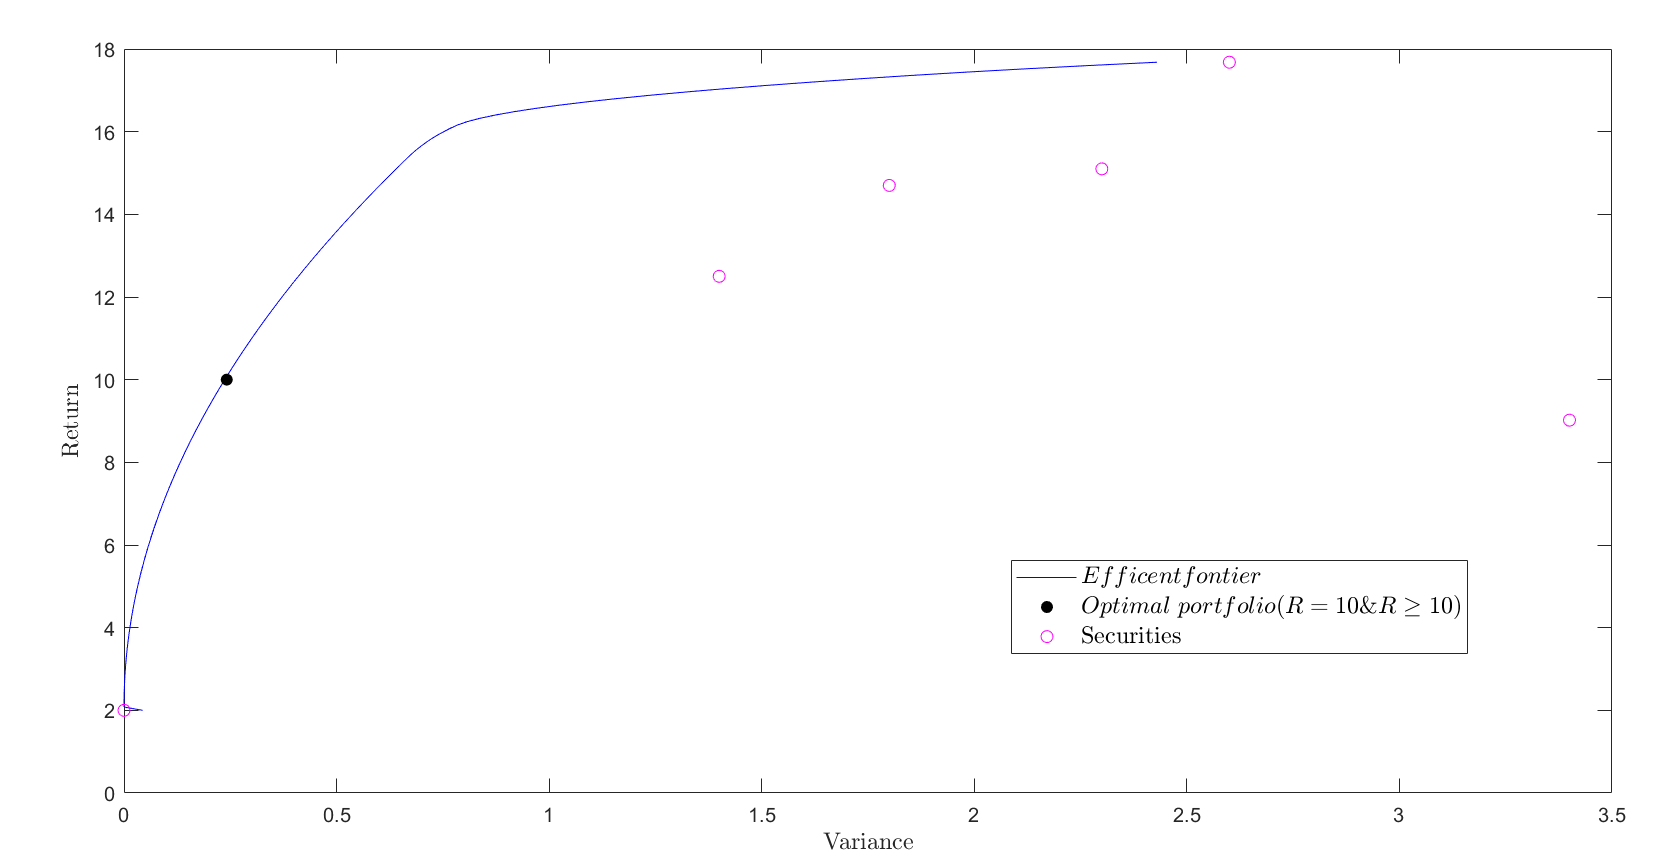
\includegraphics[scale=0.5]{figures/eff_fro2.PNG}
\caption{Efficient frontier with optimal
portfolio when $R=10$}
\label{fig:labe3.2.2}
\end{figure}
It can be seen that regardless of whether $R \ge 10$ or $R=10$, the same solution will be obtained(the black filled point). The reason can be found in the efficient frontier. After adding a risk free security, it is found that the efficient frontier increases monotonously. That is to say, when a portfolio with a higher return than or equal to a specific value and require minimum variance is desired, the variance corresponding to the higher return value is smaller than the variance corresponding to this asked return value cannot be found. Please see the driver files in appendix \ref{6.3.4}.


%%%%%%%%%%%%%%%%%%%%%%%%%%%%%%%%%%%%%%%%%%
%%%%%%%%%%%%%%%%%%%%%%%%%%%%%%%%%%%%%%%%%%%%%%%%%%%%%%%%%%%%%%%%%%%%%%%%%%%%%%%%%%%%%
%%%%%%%%%%%%%%%%%%%%%%%%%%%%%%%%%%%%%%%%%%%
%%%%%%%%%%%%%%%%%%%%%%%%%%%%%%%%%%%%%%%%%%
%%%%%%%%%%%%%%%%%%%%%%%%%%%%%%%%%%%%%%%%%%%
\subsubsection{\bfseries Optimal portfolio when $R=15$}
\begin{shaded}
{ Question: What is the minimal risk and optimal portfolio giving a return of $R = 15.00$. Plot
this point in your optimal portfolio as function of return as well as on the efficient
frontier diagram.}
\end{shaded}
when $R=15.00$ or $R\ge 15.00$
\begin{align*}
&    x=(0.1655,0.1365,0.3115,0.0266,0.3352,0.0247)^{\prime}\\
&Return: \quad E\{ R\}=15.00\\
&Risk(Variance):\quad V\{ R\}=x^{\prime}Hx=0.6383
\end{align*}
\begin{figure}[H]
\centering
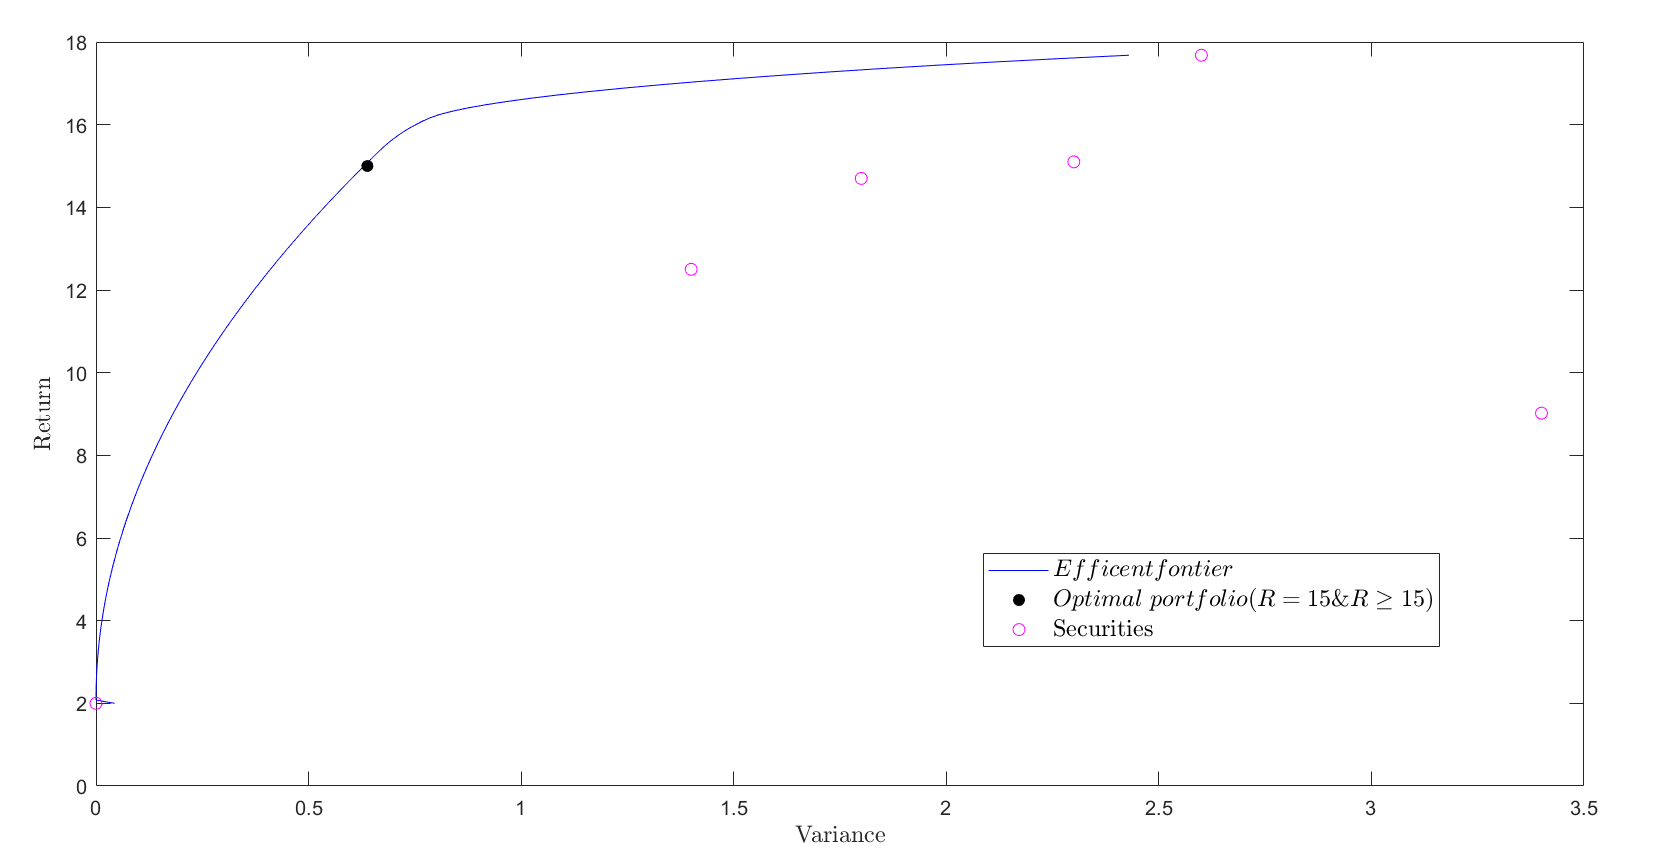
\includegraphics[scale=0.5]{figures/eff_fro3.PNG}
\caption{Efficient frontier with optimal
portfolio when $R=15$ }
\label{fig:labe3.2.2}
\end{figure}
Where the black filled dot is the optimal  portfolio when $R=10$ or $R=15$, and the pink unfilled dot is the securities.
